% ===========================================================================
% MetaCTI: Metadata-Private Cyber Threat Intelligence Sharing
%          via Anonymous Write Protocols
%
% LaTeX-Vorlage  |  Version 0.1  |  April 2026
% ---------------------------------------------------------------------------
% Zielkonferenz: USENIX Security / ACM CCS / IEEE S&P
%
% Kompilieren:
%   pdflatex metacti_paper.tex
%   bibtex   metacti_paper
%   pdflatex metacti_paper.tex
%   pdflatex metacti_paper.tex
% ---------------------------------------------------------------------------
% TODO-Marker im Text: \todo{...}   (werden in red als Box angezeigt)
% ---------------------------------------------------------------------------

% ---------------------------------------------------------------------------
% DOCUMENT CLASS
% Für USENIX Security: \documentclass[letterpaper,twocolumn,10pt]{article}
%   + \usepackage{usenix2019_v3}
% Für ACM CCS:         \documentclass[sigconf]{acmart}
% Für IEEE S&P:        \documentclass[conference]{IEEEtran}
%
% Diese Vorlage nutzt einen generischen Stil, der leicht angepasst werden
% kann. Kommentiere die nicht benötigte Klasse aus.
% ---------------------------------------------------------------------------
\documentclass[letterpaper,twocolumn,10pt]{article}

% ---------------------------------------------------------------------------
% PACKAGES
% ---------------------------------------------------------------------------
\usepackage[utf8]{inputenc}
\usepackage[T1]{fontenc}
\usepackage{microtype}           % besseres Textlayout
\usepackage{lmodern}

% Seitenlayout (USENIX-ähnlich: 1 inch margins)
\usepackage[top=1in, bottom=1in, left=1in, right=1in]{geometry}

% Mathematik
\usepackage{amsmath, amssymb, amsthm}

% Kryptografie-Notation (eigene Definitionen – kein externes crypto.sty nötig)

% Tabellen
\usepackage{booktabs}
\usepackage{multirow}
\usepackage{array}
\usepackage{tabularx}

% Grafiken & Diagramme
\usepackage{graphicx}
\usepackage{tikz}
\usetikzlibrary{arrows.meta, positioning, shapes.geometric, fit, backgrounds}
\usepackage{pgfplots}
\pgfplotsset{compat=1.18}

% Algorithmen / Protokollboxen (ohne algorithm2e)
\usepackage{float}
\usepackage{fancyvrb}
% Einfache Algorithm-Umgebung als nummeriertes Float
\usepackage{mdframed}
\newfloat{algorithm}{tbp}{loa}
\floatname{algorithm}{Algorithm}
\newcounter{algline}
% Makros für Pseudocode-Zeilen
\newcommand{\KwIn}[1]{\textbf{Input:} #1\\}
\newcommand{\KwOut}[1]{\textbf{Output:} #1\\[2pt]}
\newcommand{\KwIf}[1]{\textbf{if} #1 \textbf{then}}
\newcommand{\KwElse}{\textbf{else}}
\newcommand{\KwFor}[1]{\textbf{for} #1 \textbf{do}}
\newcommand{\BlankLine}{\\[2pt]}
\newcommand{\tcp}[1]{\hfill\textit{\small// #1}}

% Aufzählungen
\usepackage{enumitem}
\usepackage{xspace}

% Hyperlinks (letztes Package laden)
\usepackage[colorlinks=true,
            linkcolor=blue,
            citecolor=blue,
            urlcolor=blue,
            bookmarks=true]{hyperref}

% Literaturverzeichnis
\usepackage[numbers,sort&compress]{natbib}

% Kommentare / TODOs (für Entwurfsphase)
\usepackage{xcolor}
\usepackage[colorinlistoftodos,textwidth=2cm]{todonotes}
\newcommand{\TODO}[1]{\todo[color=red!30,inline]{\textbf{TODO:} #1}}
\newcommand{\NOTE}[1]{\todo[color=blue!20,inline]{\textbf{NOTE:} #1}}
\newcommand{\VERIFY}[1]{\todo[color=orange!40,inline]{\textbf{VERIFY:} #1}}

% Theorem-Umgebungen
\newtheorem{theorem}{Theorem}
\newtheorem{lemma}[theorem]{Lemma}
\newtheorem{definition}{Definition}
\newtheorem{proposition}[theorem]{Proposition}
\newtheorem{corollary}[theorem]{Corollary}

% ---------------------------------------------------------------------------
% CUSTOM COMMANDS
% ---------------------------------------------------------------------------
\newcommand{\metacti}{\textsc{MetaCTI}}
\newcommand{\express}{\textsc{Express}}
\newcommand{\riposte}{\textsc{Riposte}}
\newcommand{\taxii}{\textsc{Taxii}}
\newcommand{\misp}{\textsc{Misp}}
\newcommand{\stix}{\textsc{Stix}}
\newcommand{\tlp}[1]{\texttt{TLP:#1}}
\newcommand{\ioc}{IoC}
\newcommand{\ttp}{TTP}
\newcommand{\isac}{ISAC}
\newcommand{\cti}{CTI}

% Kryptografische Notation
\newcommand{\adv}{\mathcal{A}}
\newcommand{\negl}{\mathsf{negl}}
\newcommand{\secparam}{\lambda}
\newcommand{\xorb}{\oplus}
\newcommand{\prf}{\mathsf{PRF}}
\newcommand{\dpf}{\mathsf{DPF}}
\newcommand{\pir}{\mathsf{PIR}}
\newcommand{\zkp}{\mathsf{ZKP}}
\newcommand{\shares}[2]{\langle #1 \rangle_{#2}}
\newcommand{\sample}{\xleftarrow{\$}}   % uniform random sampling arrow

% Abkürzungen
\newcommand{\ie}{\textit{i.e.},\xspace}
\newcommand{\eg}{\textit{e.g.},\xspace}
\newcommand{\etal}{\textit{et al.}\xspace}

% Spaltentrennlinie
\setlength{\columnsep}{0.25in}

% ---------------------------------------------------------------------------
% TITLE & AUTHORS
% ---------------------------------------------------------------------------
\title{
  \textbf{\metacti: Metadata-Private Cyber Threat Intelligence Sharing\\
  via Anonymous Write Protocols}
}

\author{
  \textit{[Autoren anonymisiert für Double-Blind-Review]}
  \\[1ex]
  % Nach Deanonymisierung:
  % Vorname Nachname\textsuperscript{1} \quad
  % Vorname Nachname\textsuperscript{2}\\[0.5ex]
  % \textsuperscript{1}Institution, Land \quad
  % \textsuperscript{2}Institution, Land\\
  % \texttt{\{email1, email2\}@institution.edu}
}

\date{}   % kein Datum im Paper

% ===========================================================================
\begin{document}
\maketitle
% ===========================================================================


% ---------------------------------------------------------------------------
% ABSTRACT
% ---------------------------------------------------------------------------
\begin{abstract}
Cyber Threat Intelligence (CTI) sharing is a cornerstone of collective
cyberdefense, yet widespread adoption is hindered by a fundamental
\emph{metadata problem}: an organization that submits an Indicator of
Compromise (IoC) necessarily reveals that it has been compromised.
This metadata leakage—who shares what, when, and with whom—is often
more sensitive than the IoC itself.
Existing systems, including TAXII+TLS, MISP over Tor, and
blockchain-based approaches, protect content confidentiality but
provide no formal guarantees against communication-metadata exposure.

We present \metacti, the first CTI-sharing system with
\emph{cryptographically proven sender anonymity and metadata privacy}.
\metacti\ adapts the \express\ anonymous write protocol
(Eskandarian~\etal, USENIX~Security~2021)
to the CTI domain through four non-trivial contributions:
(i)~a formal threat model for CTI metadata leakage;
(ii)~a dual-mode architecture that eliminates costly Private Information
Retrieval (PIR) for broadcast-mode sharing (\tlp{WHITE}/\tlp{GREEN}),
reducing server compute overhead from $O(N \cdot M)$ to zero for the
common case;
(iii)~a chunking scheme with formal anonymity proofs for large
STIX objects; and
(iv)~an abuse-prevention layer combining Eskandarian's secret-sharing
abuse-reporting mechanism~\cite{eskandarian2024abuse} with
zero-knowledge membership proofs, enabling accountability without
breaking anonymity.

We implement a prototype and evaluate it against realistic CTI
workloads derived from public MISP community feeds.
\metacti\ in broadcast mode supports ISACs with up to \VERIFY{$N=500$}
members with practical bandwidth overhead; directed mode scales to
\VERIFY{$N=200$} participants before PIR becomes the bottleneck.
Compared to vanilla TAXII, the privacy cost per organization is
\VERIFY{$\approx$3\,MB/day in uplink dummy traffic} and
\VERIFY{$\approx$144\,MB/day in DB-download overhead} for a 100-member
ISAC—well within the operational capacity of modern security teams.
\end{abstract}

% ---------------------------------------------------------------------------
% SECTION 1: INTRODUCTION
% ---------------------------------------------------------------------------
\section{Introduction}
\label{sec:intro}

Collective cyberdefense depends on organizations sharing information
about threats they observe: IP addresses hosting malware, file hashes
of ransomware payloads, command-and-control domains, and behavioral
TTPs. ISACs (Information Sharing and Analysis Centers), CERTs, and
platforms such as MISP and TAXII provide the infrastructure for this
exchange. Despite clear benefits, participation remains limited.
ENISA and CISA consistently identify \emph{trust and privacy concerns}
as the primary barriers~\cite{enisa_cti_barriers,cisa_sharing}.

The root cause is not a lack of willingness, but a structural
\emph{metadata exposure problem}:

\begin{quote}
  \emph{An organization that submits an IoC reveals that it has been
  compromised.}
\end{quote}

This is harmful in multiple ways. Adversaries learn which of their
techniques were detected and can rotate TTPs before other victims
respond. Regulators, competitors, and media can observe security
incidents in near real time from submission timestamps. Even the
\emph{frequency} of submissions leaks information about an
organization's threat exposure.

Current defenses are insufficient. TAXII over TLS encrypts payloads
but exposes who connects to whom and when. MISP over
Tor~\cite{wagner2018} hides IP addresses but provides no formal
anonymity guarantees against active attackers or timing-correlation
attacks. Blockchain-based approaches~\cite{TODO_blockchain_cti} offer
pseudonymity while making the transaction graph and timestamps
permanently public. The most recent academic system, SeCTIS~2024, uses
federated swarm learning and explicitly calls \emph{connection
anonymity} an open research question~\cite{alsaedi2024sectis}.

\textbf{Our approach.} We observe that the anonymous-messaging
community has solved an analogous problem: how can a whistleblower
submit information to a server without revealing their identity to the
server or a network observer? The \express\ protocol of
Eskandarian~\etal~\cite{eskandarian2021express} achieves this via a
two-server XOR secret-sharing scheme, providing cryptographically
provable sender anonymity with write costs of only $2M$ bytes per
client per round—independent of the number of participants $N$.

Adapting \express\ to CTI is non-trivial. CTI objects are large and
heterogeneous (STIX bundles range from $<$1\,KB to several MB), sharing
is asynchronous and event-driven rather than synchronous,
TLP-based access control requires multiple sharing modes with different
privacy guarantees, and anonymous submission opens new attack surfaces
for false-positive and poisoning attacks.

\textbf{Contributions.} We make four contributions:

\begin{enumerate}[leftmargin=*,nosep]
  \item \textbf{Formal Threat Model (§\ref{sec:threat_model}).}
    We define the first formal adversary model for CTI metadata leakage,
    classifying existing systems against it.

  \item \textbf{Dual-Mode Protocol Design (§\ref{sec:protocol}).}
    \metacti\ separates broadcast-mode (\tlp{WHITE}/\tlp{GREEN}) from
    directed-mode (\tlp{AMBER}/\tlp{RED}) sharing. Broadcast mode
    eliminates PIR entirely; directed mode uses DPF-based PIR only where
    reader anonymity is required.

  \item \textbf{Abuse Prevention (§\ref{sec:abuse}).}
    We integrate Eskandarian's abuse-reporting mechanism with
    ZKP-based sector-membership proofs to enable accountability under
    full sender anonymity.

  \item \textbf{Implementation \& Evaluation (§\ref{sec:eval}).}
    We build a prototype in Python/Rust, characterize real-world CTI
    workloads, and provide concrete deployment guidelines.
\end{enumerate}

\textbf{Ethical considerations.} \TODO{Ablehnung des DC-Netz-Hybrids
begründen (Sicherheitsargument), IRB-Hinweis für Nutzer-Befragungen,
Open-Source-Release-Plan.}


% ---------------------------------------------------------------------------
% SECTION 2: BACKGROUND
% ---------------------------------------------------------------------------
\section{Background}
\label{sec:background}

\subsection{CTI Sharing Standards: STIX and TAXII}
\label{sec:stix_taxii}

STIX (Structured Threat Information eXpression)~2.1~\cite{stix21} is
the de-facto standard for representing CTI as JSON-based objects.
Key object types include \texttt{indicator} (IoCs such as IPs, hashes,
domains), \texttt{malware}, \texttt{attack-pattern}, \texttt{course-of-action},
and \texttt{report}. STIX objects are exchanged as \emph{bundles}.
Object sizes span several orders of magnitude:
individual IoC indicators are typically 0.5–2\,KB;
reports with YARA rules reach 30–300\,KB;
large incident bundles with disassembly traces may exceed 1\,MB
(\S\ref{sec:chunking}).

TAXII~2.1~\cite{taxii21} defines a client–server REST API for STIX
distribution. It provides content confidentiality via TLS but no
protection for communication metadata.

The \emph{Traffic Light Protocol (TLP)} defines four sharing levels:
\tlp{WHITE} (unrestricted), \tlp{GREEN} (community-wide),
\tlp{AMBER} (recipient-limited), and \tlp{RED} (bilateral).
These levels impose fundamentally different privacy requirements—a
distinction that \metacti's dual-mode architecture directly encodes.

\subsection{The EXPRESS Protocol}
\label{sec:express}

\express~\cite{eskandarian2021express} is a metadata-hiding
communication system for anonymous bulletin boards. We summarize the
components relevant to \metacti.

\textbf{Write protocol (Secret Sharing).}
A client wishing to write message $M$ of length $|M|$ bytes into
mailbox $i$:
\begin{enumerate}[nosep]
  \item generates a uniformly random string $S$ of length $|M|$;
  \item sends the share $(i,\; S)$ to Server~1;
  \item sends the share $(i,\; S \xorb M)$ to Server~2.
\end{enumerate}
Each server writes its share into its local copy of mailbox~$i$.
The original message is recovered by XOR-combining both shares:
$S \xorb (S \xorb M) = M$.

No single server observes $M$. Under the assumption that the two
servers do not collude, neither learns the message content nor the
true mailbox index $i$ (because each share is computationally
indistinguishable from random).\footnote{More precisely, \express\
uses a PRF-based share-generation mechanism that also allows the servers
to \emph{audit} that a client has written well-formed content into
exactly one mailbox, providing protection against disruptive
participants~\cite{corrigan2015riposte}.}

\textbf{Write cost:} $2|M|$ bytes per client per round,
\emph{independent of} the number of mailboxes $N$.
This is the key improvement over \riposte~\cite{corrigan2015riposte},
which requires $O(N \cdot |M|)$ per client.

\textbf{Read protocol (PIR).}
To read mailbox $j$ without revealing $j$ to the servers, a client
uses Distributed Point Functions (DPF)-based Private Information
Retrieval:
\begin{itemize}[nosep]
  \item Client sends two DPF queries (each $O(\secparam \cdot \log N)$
        bytes) to the servers.
  \item Each server evaluates the query over its copy of the full
        database: $O(N \cdot |M|)$ compute.
  \item Each server returns one response of size $|M|$.
  \item Client reconstructs mailbox $j$ by XOR-combining the responses.
\end{itemize}
The PIR guarantee: no server learns which mailbox was queried.
\emph{PIR server compute} is the primary scalability bottleneck in the
read path.

\subsection{Related Work}
\label{sec:related}

\TODO{Vollständige Related-Work-Sektion; wichtige Punkte sind in notes.md
§1.2 und §10. Tabelle~\ref{tab:comparison} zeigt Systemvergleich.}

Table~\ref{tab:comparison} classifies prior CTI sharing systems along
the dimensions of our formal threat model (§\ref{sec:threat_model}).

\begin{table*}[t]
\centering
\caption{Comparison of CTI sharing systems. \checkmark~=~provided,
(\checkmark)~=~partially, \texttimes~=~not provided, n/a~=~not
applicable.}
\label{tab:comparison}
\renewcommand{\arraystretch}{1.2}
\begin{tabular}{lcccccc}
\toprule
\textbf{System} &
\textbf{Content Privacy} &
\textbf{Sender Anonymity} &
\textbf{Metadata Privacy} &
\textbf{Abuse Prevention} &
\textbf{Formal Guarantees} &
\textbf{Scalability} \\
\midrule
TAXII + TLS              & \checkmark & \texttimes        & \texttimes   & n/a             & \texttimes & High   \\
MISP + Tor~\cite{wagner2018}
                         & \checkmark & Weak              & Weak         & n/a             & \texttimes & Medium \\
Blockchain CTI           & \checkmark & Pseudonym         & \texttimes   & \texttimes      & \texttimes & Low    \\
Huff~\etal~\cite{huff2024}
                         & \checkmark & vs.\ receiver     & \texttimes   & \texttimes      & (\checkmark) & Medium \\
SeCTIS 2024~\cite{alsaedi2024sectis}
                         & \checkmark (FL) & \texttimes   & \texttimes   & \checkmark      & (\checkmark) & Medium \\
FL+DP (Fischer~\cite{fischer_eth})
                         & \checkmark & \texttimes        & \texttimes   & \texttimes      & \checkmark & Medium \\
\midrule
\textbf{\metacti (ours)} & \checkmark & \textbf{\checkmark} (crypto.) &
\textbf{\checkmark} (formal) & \textbf{\checkmark} & \textbf{\checkmark} & Medium \\
\bottomrule
\end{tabular}
\end{table*}

\textbf{Anonymous messaging systems.}
\riposte~\cite{corrigan2015riposte} introduced the $k$-server audit
approach for write-private databases.
\express~\cite{eskandarian2021express} reduces write cost from
$O(N)$ to $O(1)$ (in $N$) using a two-server model.
Dissent~\cite{corrigan2010dissent} (accountable DC-nets) was the
predecessor to \riposte; we explicitly \emph{do not} adopt a DC-net
hybrid (§\ref{sec:design_decisions}).

\textbf{CTI sharing.}
Wagner~\etal~\cite{wagner2018} were the first to apply anonymization
to CTI sharing via MISP over Tor;
our system provides formal guarantees that Tor cannot.
SeCTIS~\cite{alsaedi2024sectis} explicitly lists \emph{connection
anonymity} as future work—exactly the gap \metacti\ fills.
Huff~\etal~\cite{huff2024} protect submitter identity from the
\emph{recipient} using BBS+ credentials but not from the infrastructure.


% ---------------------------------------------------------------------------
% SECTION 3: THREAT MODEL
% ---------------------------------------------------------------------------
\section{Threat Model}
\label{sec:threat_model}

\subsection{System Model}

A \metacti\ deployment consists of:
\begin{itemize}[nosep]
  \item $N$ \emph{participants} (organizations, ISAC members), each
        holding a membership credential for the sharing community.
  \item Two \emph{servers} $S_1$ and $S_2$, operated by distinct legal
        entities (e.g., a national CERT and an independent security
        research institute).
  \item An optional \emph{encrypted object store} for out-of-band
        transfer of large objects (§\ref{sec:chunking}).
\end{itemize}

\subsection{Adversary Model}

We consider three adversary types:

\begin{definition}[Honest-but-Curious Server]
  A server $S_i$ follows the protocol faithfully but attempts to infer
  as much as possible about participants' identities and behavior from
  all data it observes, including timing.
\end{definition}

\begin{definition}[Malicious Participant]
  A subset of at most $t$ participants deviate arbitrarily from the
  protocol, attempt to identify honest participants, and may inject
  false data.
\end{definition}

\begin{definition}[Passive Network Observer]
  An adversary who monitors all network links, can observe packet
  sizes and timing, but cannot break TLS or decrypt payloads.
\end{definition}

We additionally define a \emph{colluding-server adversary} as out of
scope: our two-server construction relies on non-collusion
(§\ref{sec:trust_model}).

\subsection{Security Goals}

\begin{definition}[Sender Anonymity]
  For any two organizations $\mathcal{O}_0, \mathcal{O}_1$ and any
  STIX object $m$, no p.p.t. adversary $\adv$ can distinguish whether
  $\mathcal{O}_0$ or $\mathcal{O}_1$ submitted $m$ with probability
  greater than $\frac{1}{2} + \negl(\secparam)$.
  Formally, this is captured as an indistinguishability game
  $\mathsf{SenderAnon}_{\adv}^{\metacti}(\secparam)$.
\end{definition}

\begin{definition}[Reader Anonymity]
  (Directed mode only.) No server can link a PIR query to the
  requesting organization beyond what is implied by membership in the
  sharing community.
\end{definition}

\begin{definition}[Unlinkability]
  Submissions by the same organization across rounds cannot be
  correlated, even given traffic-volume information.
\end{definition}

\begin{definition}[Submission Integrity]
  All accepted STIX objects originate from legitimate ISAC members,
  and the system can—upon reported abuse—deanonymize a specific
  submitter without affecting others' anonymity.
\end{definition}

\subsection{Metadata Leakage Taxonomy}

\TODO{Tabelle: welche Metadaten gibt welches System preis? Spalten:
sender IP, timing, submission frequency, submission count, sector
membership, IOC type. Zeilen: TAXII, MISP+Tor, Blockchain, \metacti.}

We identify four classes of CTI-specific metadata leakage attacks:

\textbf{L1 – Sender identification:} The server or a network observer
determines which organization submitted IoC $x$.

\textbf{L2 – Timing inference:} The timestamp of a submission reveals
when an incident occurred.

\textbf{L3 – Volume profiling:} Unusually high submission frequency
indicates an active, ongoing incident.

\textbf{L4 – TTP exposure:} The \emph{type} of IoC submitted reveals
which TTPs were detected, enabling adversarial rotation.

\subsection{Out-of-Scope Threats}

We do not address: (a) side-channel attacks against participant
hardware; (b) content-level analysis of shared STIX objects;
(c) server compromise (mitigated by the non-collusion assumption);
(d) active network attacks that selectively block server connections.

\subsection{Trust Model}
\label{sec:trust_model}

The two-server non-collusion assumption is the fundamental trust
requirement. In practice, this can be achieved by:
\begin{itemize}[nosep]
  \item Placing the two servers in different legal jurisdictions
        (subpoenas cannot easily span both).
  \item Assigning operation to: a national CERT + an independent
        security research institute; or two competing ISACs.
\end{itemize}
\TODO{Governance-Diskussion ausweiten; Referenz auf ähnliche
Zwei-Server-Deployments in der Praxis (Signal, CONIKS, etc.)}


% ---------------------------------------------------------------------------
% SECTION 4: PROTOCOL DESIGN
% ---------------------------------------------------------------------------
\section{MetaCTI Protocol Design}
\label{sec:protocol}

\subsection{Overview and Design Rationale}

\metacti\ adapts \express\ to the CTI domain along four dimensions:
(i) \emph{dual-mode architecture} to exploit the absence of a read-privacy
requirement in broadcast-mode CTI sharing;
(ii) \emph{chunking} for large STIX objects with formal anonymity
preservation;
(iii) \emph{asynchronous round management} with dummy-traffic scheduling;
(iv) \emph{TLP-based access control} within the directed-mode.

\textbf{Key design decision: No DC-net hybrid.}
\label{sec:design_decisions}
An early design candidate used \express\ only for write verification
and a DC-net for actual data transfer, exploiting DC-nets' lower send
cost ($M$ vs. $2M$ per client).
We rejected this for three reasons:
(1) \express' verification is tightly coupled to its secret-sharing
construction; separating them requires building a second protocol
(essentially Dissent~\cite{corrigan2010dissent}, which proved too slow
for practical use);
(2) the net bandwidth saving ($M$ vs. $2M$) is consumed by the
verification phase overhead;
(3) DC-nets require all-to-all connectivity, which is unrealistic in
ISAC environments with strict firewall policies.

\subsection{Dual-Mode Architecture}
\label{sec:dual_mode}

The central observation enabling our dual-mode design is:

\begin{quotation}
  \noindent\emph{In broadcast-mode CTI sharing (\tlp{WHITE}/\tlp{GREEN}),
  reader anonymity is not a goal—every participant should know
  everything. Only sender anonymity must be protected.
  Therefore, PIR is unnecessary.}
\end{quotation}

This simple observation has significant performance implications.

\textbf{\metacti-Broadcast (\tlp{WHITE}/\tlp{GREEN}).}
After each round:
\begin{enumerate}[nosep]
  \item All $N$ clients submit a write share or a dummy write.
  \item Both servers reconstruct the full database $\mathsf{DB}$.
  \item $\mathsf{DB}$ is published as a static snapshot.
  \item All clients download $\mathsf{DB}$ in full.
\end{enumerate}
PIR is completely absent. The read path is equivalent to a CDN-hosted
file download; the full server-side compute overhead of $O(N \cdot M)$
per PIR query is eliminated.

\textbf{\metacti-Directed (\tlp{AMBER}/\tlp{RED}).}
Mailboxes in the directed-mode database correspond to recipient groups
(e.g., all members of the financial-sector sub-ISAC, or a bilateral
pair). Recipients read only their group mailbox via DPF-PIR:
\begin{enumerate}[nosep]
  \item Client submits encrypted write shares with group-key-based
        payload encryption.
  \item Recipients read their group mailbox via PIR to preserve
        reader anonymity.
  \item PIR queries reveal only that the client is a community member,
        not which mailbox is accessed.
\end{enumerate}

\TODO{Formale Beschreibung des Group-Mailbox-Schemas; Schlüssel-
Verteilung für Gruppen-Keys.}

\begin{figure}[t]
\centering
% TODO: TikZ-Diagramm der Dual-Mode-Architektur hier einfügen
% Vorlage für TikZ-Architektur:
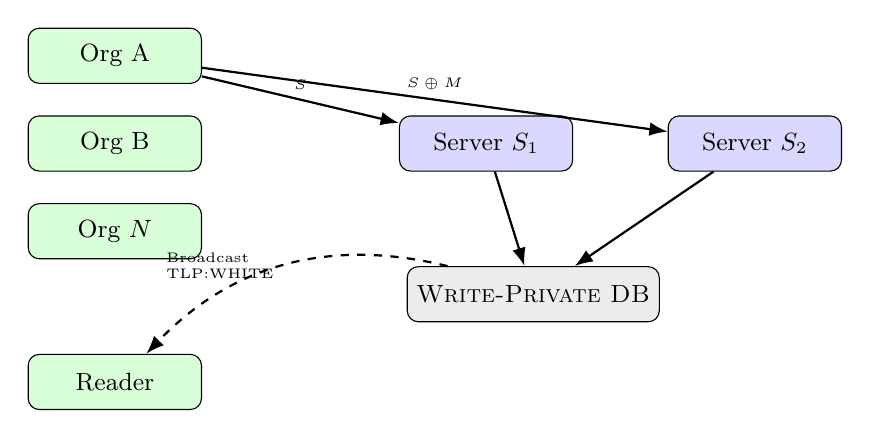
\begin{tikzpicture}[
  node distance=1.5cm and 2cm,
  box/.style={rectangle, draw, rounded corners, minimum width=2.2cm,
              minimum height=0.7cm, font=\small},
  server/.style={box, fill=blue!15},
  client/.style={box, fill=green!15},
  db/.style={box, fill=gray!15},
  arrow/.style={-{Latex}, thick}
]
  \node[client] (orgA) {Org A};
  \node[client, below=0.4cm of orgA] (orgB) {Org B};
  \node[client, below=0.4cm of orgB] (orgN) {Org $N$};
  \node[server, right=2.5cm of orgB] (s1) {Server $S_1$};
  \node[server, right=1.2cm of s1] (s2) {Server $S_2$};
  \node[db, below=1.2cm of s1, xshift=0.6cm] (db) {\textsc{Write-Private DB}};
  \node[client, below=1.2cm of orgN] (reader) {Reader};

  \draw[arrow] (orgA) -- node[above,font=\tiny]{$S$} (s1);
  \draw[arrow] (orgA) -- node[above,font=\tiny]{$S\xorb M$} (s2);
  \draw[arrow] (s1) -- (db);
  \draw[arrow] (s2) -- (db);

  % Broadcast path
  \draw[arrow, dashed] (db) to[bend right=30]
    node[left,font=\tiny,align=left]{Broadcast\\TLP:WHITE} (reader);

\end{tikzpicture}
\caption{\metacti\ dual-mode architecture. Solid lines show the
write path (secret-sharing). Dashed line shows broadcast-mode
public DB download (no PIR). Directed-mode (not shown) uses
DPF-PIR for the read path.}
\label{fig:architecture}
\end{figure}

\subsection{Round Structure and Timing}
\label{sec:rounds}

\metacti\ operates in synchronized rounds of duration $\Delta t$.
Choosing $\Delta t$ involves a fundamental trade-off:

\begin{itemize}[nosep]
  \item \textbf{Shorter rounds} ($\Delta t = 1$–5\,min): lower IoC
        dissemination latency, higher dummy-traffic volume.
  \item \textbf{Longer rounds} ($\Delta t = 10$–30\,min): lower
        dummy-traffic cost, acceptable for strategic threat reports.
\end{itemize}

\VERIFY{Empirische Validierung der akzeptablen Latenz durch
Befragung von CTI-Praktikern. Vorläufige Annahme: 5–15\,min für
operative IoCs; 30–60\,min für strategische Reports.}

\subsection{Dummy-Traffic Scheduling}
\label{sec:dummy}

In every round, each participant must submit \emph{something}—either
a genuine STIX object or a dummy write (random bits, indistinguishable
from a real share). Failure to submit in a round leaks a binary bit:
``this participant had nothing to share.'' Over time, this enables
volume-profiling attacks (L3, §\ref{sec:threat_model}).

\textbf{Scheduler design.}
The dummy-traffic scheduler ensures:
\begin{enumerate}[nosep]
  \item \emph{Participation obligation}: every registered member
        submits exactly one write per round.
  \item \emph{Timing smoothing}: genuine writes are not distinguishable
        from dummy writes by submission timing within a round.
  \item \emph{Relaxation analysis}: \TODO{Formal zu zeigen: Dürfen
        Clients $k$ aus $n$ Rounds aussetzen ohne
        Traffic-Volume-Angriffe zu ermöglichen? Vgl. notes.md §8.1.}
\end{enumerate}

\subsection{Chunking for Large STIX Objects}
\label{sec:chunking}

\express\ was designed for fixed-size messages. STIX objects span
several orders of magnitude. We adopt a three-tier scheme:

\textbf{Tier 1 ($< M_{\text{slot}}$, default: 32\,KB).}
Direct \express\ write. No additional overhead.

\textbf{Tier 2 ($M_{\text{slot}}$–1\,MB).}
Object is fragmented into $\lceil |M|/M_{\text{slot}} \rceil$ chunks.
Chunks are symmetrically encrypted with a per-object session key $k$.
The first chunk contains a header with key $k$ and total chunk count.
Subsequent chunks are written in subsequent rounds into pseudo-randomly
selected slots (seeded by a commitment to $k$).

\textbf{Tier 3 ($>$1\,MB).}
Object is encrypted with key $k$ and stored on a separate
encrypted object store (S3-compatible). Only a small STIX reference
object ($<$1\,KB) containing the URL and $k$ is transmitted via
\metacti. The out-of-band download is not anonymous but reveals
nothing about content (ciphertext only).

\textbf{Slot size selection.}
We choose $M_{\text{slot}} = 32$\,KB based on:
\begin{itemize}[nosep]
  \item Covers $\approx$90\% of operational IoC sharing without chunking
        (empirically validated in §\ref{sec:workload}).
  \item Database size: $N=100$ members $\times$ 32\,KB $=$ 3.2\,MB per round,
        practical for public download.
  \item Power-of-two size simplifies implementation alignment.
\end{itemize}

\begin{theorem}[Chunking Anonymity Preservation]
  Multi-round chunking with pseudo-random slot assignment does not
  introduce cross-round timing correlations that break sender anonymity
  under the \express\ non-collusion assumption.
\end{theorem}
\begin{proof}
  \TODO{Formaler Beweis. Kern-Argument: Slot-Auswahl für Chunks ist
  PRF-basiert und committet nur in der ersten Runde; keine
  Korrelation zwischen aufeinanderfolgenden Runden ohne Kenntnis von
  $k$. Vgl. notes.md §6.3.}
\end{proof}

\subsection{Protocol Specification}
\label{sec:protocol_spec}

\TODO{Formale Protokollbeschreibung als Algorithm-Umgebung.
Vorlage unten.}

\begin{algorithm}[t]
\caption{\metacti-Broadcast: Write Protocol}
\label{alg:write_broadcast}
\begin{mdframed}[linewidth=0.4pt, innerleftmargin=6pt,
                 innerrightmargin=6pt, innertopmargin=4pt,
                 innerbottommargin=4pt]
\KwIn{Message $M \in \{0,1\}^*$, slot $i \in [N]$, servers $S_1, S_2$}
\KwOut{Anonymous write into slot $i$}
\begin{enumerate}[label=\arabic*:, nosep, leftmargin=2em]
  \item \KwIf{$|M| \leq M_{\text{slot}}$}
  \item \quad $M' \leftarrow M \mathbin\| 0^{M_{\text{slot}} - |M|}$ \tcp{zero-pad to slot size}
  \item \quad $R \sample \{0,1\}^{M_{\text{slot}}}$
  \item \quad Send $(i,\; R)$ to $S_1$
  \item \quad Send $(i,\; R \xorb M')$ to $S_2$
  \item \KwElse\ \metacti-Chunk$(M, i)$ \tcp{Tier-2/3, see §\ref{sec:chunking}}
\end{enumerate}
\end{mdframed}
\end{algorithm}

\begin{algorithm}[t]
\caption{\metacti-Broadcast: Read Protocol}
\label{alg:read_broadcast}
\begin{mdframed}[linewidth=0.4pt, innerleftmargin=6pt,
                 innerrightmargin=6pt, innertopmargin=4pt,
                 innerbottommargin=4pt]
\KwIn{None (broadcast: full DB public)}
\KwOut{Reconstructed database $\mathsf{DB}$}
\begin{enumerate}[label=\arabic*:, nosep, leftmargin=2em]
  \item Download $\mathsf{DB}$ from public endpoint
  \item \KwFor{$j \leftarrow 1$ to $N$}
  \item \quad $\mathsf{DB}[j] \leftarrow \text{decrypt}(\mathsf{DB}[j])$
  \item \quad \KwIf{$\mathsf{DB}[j] \neq \bot$}\ parse STIX object
\end{enumerate}
\end{mdframed}
\end{algorithm}

\subsection{Security Analysis}
\label{sec:security}

\begin{theorem}[Sender Anonymity of \metacti-Broadcast]
  Under the two-server non-collusion assumption and PRF security of
  the share-generation function, \metacti-Broadcast achieves sender
  anonymity as defined in Definition~1.
\end{theorem}
\begin{proof}
  \TODO{Reduktionsbeweis auf \express-Sicherheitsaussage von
  Eskandarian~\etal~\cite{eskandarian2021express}. Zeige, dass
  CTI-Anpassungen (Padding, TLP-Labels) die Indistinguishability
  nicht verletzen.}
\end{proof}

\begin{theorem}[Sender Anonymity of \metacti-Directed]
  Under the two-server non-collusion assumption, PRF security, and
  DPF security~\cite{TODO_dpf}, \metacti-Directed achieves sender and
  reader anonymity.
\end{theorem}
\begin{proof}
  \TODO{Erweiterung des Broadcast-Beweises um PIR-Sicherheit via DPF.}
\end{proof}


% ---------------------------------------------------------------------------
% SECTION 5: ABUSE PREVENTION
% ---------------------------------------------------------------------------
\section{Abuse Prevention Under Anonymity}
\label{sec:abuse}

Strong sender anonymity introduces a new attack surface: an adversary
can inject false positives or poisoned IoCs without being
identifiable. We address this in two layers.

\subsection{Abuse Reporting via Secret Sharing}
\label{sec:abuse_reporting}

We integrate Eskandarian's abuse-reporting mechanism~\cite{eskandarian2024abuse}.
On submission, each client attaches a \emph{cryptographic report token}
$\tau$ via secret sharing across both servers. In normal operation,
$\tau$ is never reconstructed. If a recipient flags a submission as
abusive:
\begin{enumerate}[nosep]
  \item Both servers receive the abuse report.
  \item Both servers contribute their share of $\tau$ to
        reconstruct the submitter's identity.
  \item Only the flagged submitter is deanonymized; all other users'
        anonymity is preserved.
\end{enumerate}

\textbf{CTI-specific calibration.}
The abuse threshold $\theta$ (number of independent abuse reports
required before deanonymization) must balance false-positive errors
(legitimate organizations inadvertently poisoning feeds) against
false-report attacks (adversaries flagging legitimate contributions to
deanonymize competitors). We analyze this trade-off in
§\ref{sec:eval_abuse}.

\TODO{Formal: Nachweis, dass der Abuse-Reporting-Mechanismus die
Sender-Anonymität für nicht-flagged Nutzer nicht beeinträchtigt.
Direkte Übernahme aus Eskandarian 2024 möglich.}

\subsection{ZKP-Based Sector Membership Proof}
\label{sec:zkp}

To strengthen submission quality without breaking anonymity, we require
each submitter to prove membership in a legitimate ISAC sector without
revealing their identity:

\begin{definition}[Sector Membership Proof]
  An organization $\mathcal{O}$ holds a membership credential
  $\sigma$ issued by the ISAC. Before each round, $\mathcal{O}$
  produces a zero-knowledge proof $\pi$ that:
  $\exists\, \sigma$ such that $\text{Verify}(\mathsf{pk}_{\mathsf{ISAC}},
  \sigma, \mathcal{O}) = 1$ and $\mathcal{O} \in \mathsf{SectorGroup}$,
  without revealing $\mathcal{O}$.
\end{definition}

\textbf{ZKP scheme selection.}
We evaluate three candidates:
\begin{itemize}[nosep]
  \item \emph{Merkle-tree membership proof}: simple, established,
        $O(\log n)$ proof size for $n$ members.
  \item \emph{BBS+ credentials}~\cite{huff2024}: efficient for repeated
        use, supports selective disclosure.
  \item \emph{Pedersen-commitment-based}: maximally flexible,
        higher verification cost.
\end{itemize}
\VERIFY{Konkrete Wahl und Performance-Vergleich nach Implementierung.}


% ---------------------------------------------------------------------------
% SECTION 6: IMPLEMENTATION
% ---------------------------------------------------------------------------
\section{Implementation}
\label{sec:implementation}

We implement \metacti\ as an open-source prototype.\footnote{Code
will be released at \texttt{[anonymized]}.}

\subsection{Components}

\textbf{Server (Python/Rust).}
The server implementation consists of:
\begin{itemize}[nosep]
  \item Write-share collector and verifier (Rust, for performance);
  \item PIR query handler using DPF (Rust, based on the
        \express\ reference implementation~\cite{express_code});
  \item Round coordinator (Python) for round timing and DB export;
  \item Abuse-reporting endpoint.
\end{itemize}

\textbf{Client library (Python).}
\begin{itemize}[nosep]
  \item STIX 2.1 serialization/deserialization (\texttt{stix2} library);
  \item Share generation with PRF-based write construction;
  \item Chunking module (Tier 1–3);
  \item Dummy-traffic scheduler;
  \item ZKP membership proof generation.
\end{itemize}

\textbf{Integration.}
The client library exposes a TAXII-compatible API surface, enabling
drop-in replacement of existing TAXII clients.

\subsection{Engineering Challenges}

\textbf{Round synchronization.}
\TODO{NTP-basierte Synchronisierung; wie geht das System mit
Ausfällen einzelner Clients um?}

\textbf{PIR performance.}
The DPF evaluation in the directed mode requires iterating over the
full database per query. We optimize using:
\begin{itemize}[nosep]
  \item Batching multiple PIR queries per round;
  \item SIMD-accelerated XOR operations;
  \item CDN-based caching for broadcast-mode DB distribution.
\end{itemize}


% ---------------------------------------------------------------------------
% SECTION 7: EVALUATION
% ---------------------------------------------------------------------------
\section{Evaluation}
\label{sec:eval}

We address four evaluation questions:
\begin{enumerate}[label=\textbf{E\arabic*.},nosep]
  \item \emph{Workload characterization}: What are typical STIX object
        sizes and sharing frequencies in real ISACs?
  \item \emph{Performance}: What are the throughput, latency, and
        bandwidth costs of \metacti\ for realistic workloads?
  \item \emph{Scalability}: Up to what community size $N$ is
        \metacti\ practical?
  \item \emph{Abuse prevention}: What is the accuracy/cost trade-off
        of the abuse-reporting threshold?
  \label{sec:eval_abuse}
\end{enumerate}

\subsection{Workload Characterization}
\label{sec:workload}

\TODO{Messung an öffentlichen MISP Community Feeds. Erwartetes Ergebnis
laut notes.md §6.1: $\approx$90\% der Objekte < 32\,KB.}

We analyze \TODO{$X$\,thousand} STIX objects from public MISP community
feeds~\cite{TODO_misp_feeds} to characterize object sizes and sharing
frequencies.

\begin{figure}[t]
\centering
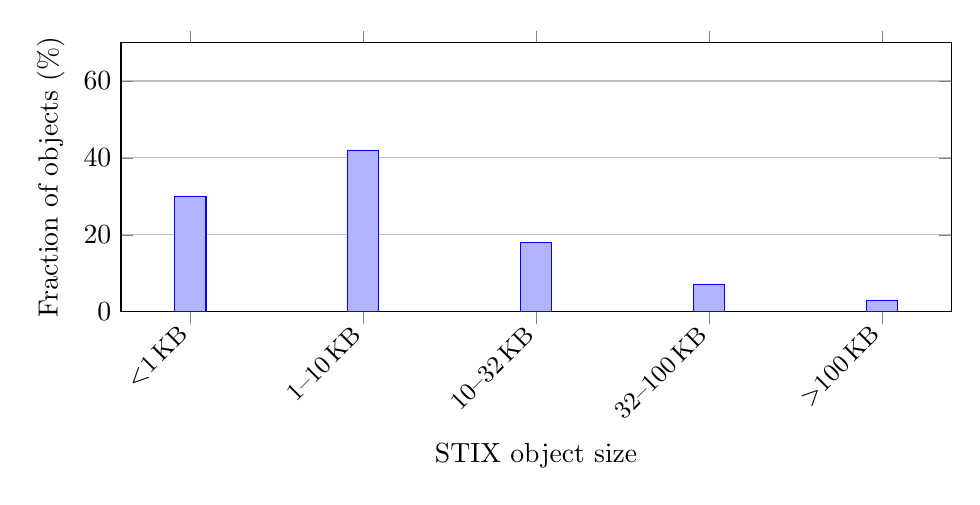
\begin{tikzpicture}
  \begin{axis}[
    ybar,
    xlabel={STIX object size},
    ylabel={Fraction of objects (\%)},
    symbolic x coords={$<$1\,KB, 1--10\,KB, 10--32\,KB,
                        32--100\,KB, $>$100\,KB},
    xtick=data,
    x tick label style={rotate=45,anchor=east,font=\small},
    bar width=0.4cm,
    ymin=0, ymax=70,
    ymajorgrids=true,
    width=\columnwidth, height=5cm,
  ]
  % TODO: mit echten Messdaten ersetzen
  \addplot coordinates {
    ($<$1\,KB, 30) (1--10\,KB, 42) (10--32\,KB, 18)
    (32--100\,KB, 7) ($>$100\,KB, 3)
  };
  \end{axis}
\end{tikzpicture}
\caption{Distribution of STIX object sizes in public MISP feeds
(preliminary / to be measured).}
\label{fig:stix_sizes}
\end{figure}

\subsection{Performance and Scalability}

\textbf{Setup.}
\TODO{Testumgebung: N Server-Nodes, Netzwerk-Emulation für verschiedene
Teilnehmergrößen.}

\textbf{Metrics.}
We measure: (i) end-to-end IoC submission latency (submission to DB
availability); (ii) per-participant bandwidth (uplink dummy traffic +
downlink DB download); (iii) server CPU and RAM load; (iv) throughput
(IoCs/round).

\begin{table}[t]
\centering
\caption{Estimated bandwidth overhead per participant per day
(broadcast mode, $\Delta t = 10$\,min, $M = 10$\,KB).
\emph{All values to be replaced by measured results.}}
\label{tab:bandwidth}
\renewcommand{\arraystretch}{1.2}
\begin{tabular}{rrrr}
\toprule
$N$ & \textbf{Dummy-Send/day} & \textbf{DB size} & \textbf{DL/day} \\
\midrule
50  & 2.88\,MB & 500\,KB & 72\,MB   \\
100 & 2.88\,MB & 1\,MB   & 144\,MB  \\
200 & 2.88\,MB & 2\,MB   & 288\,MB  \\
500 & 2.88\,MB & 5\,MB   & 720\,MB  \\
1000 & 2.88\,MB & 10\,MB & 1.44\,GB \\
\bottomrule
\end{tabular}
\end{table}

Key observation: dummy-send costs do \emph{not} scale with $N$
(the \express\ advantage over \riposte), while DB-download scales
linearly. Mitigation for large $N$: diff-based download
(only new entries since last round).

\begin{figure}[t]
\centering
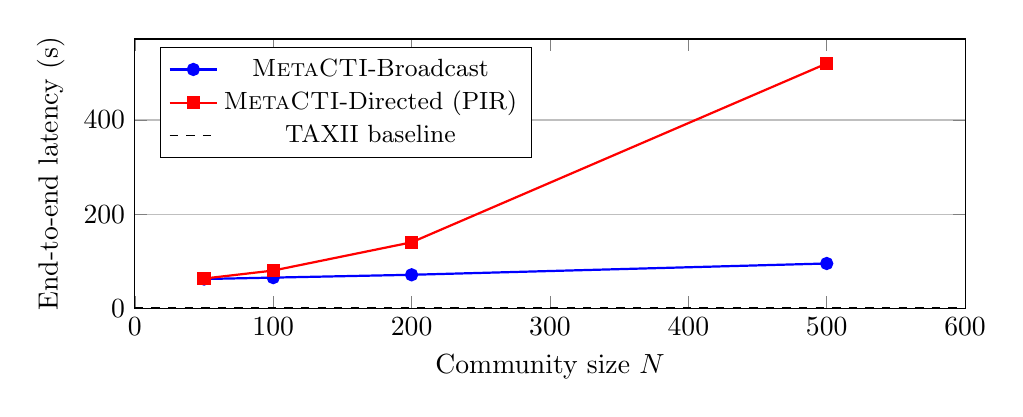
\begin{tikzpicture}
  \begin{axis}[
    xlabel={Community size $N$},
    ylabel={End-to-end latency (s)},
    xmin=0, xmax=600,
    ymin=0,
    legend pos=north west,
    legend style={font=\small},
    width=\columnwidth, height=5cm,
    ymajorgrids=true,
  ]
  % TODO: mit Messdaten ersetzen
  \addplot[blue, thick, mark=*]
    coordinates {(50,62)(100,65)(200,71)(500,95)};
  \addlegendentry{\metacti-Broadcast}
  \addplot[red, thick, mark=square*]
    coordinates {(50,63)(100,80)(200,140)(500,520)};
  \addlegendentry{\metacti-Directed (PIR)}
  \addplot[black, dashed, mark=none]
    coordinates {(0,2)(600,2)};
  \addlegendentry{TAXII baseline}
  \end{axis}
\end{tikzpicture}
\caption{End-to-end IoC dissemination latency (preliminary; to be
measured). Round duration $\Delta t = 60$\,s.}
\label{fig:latency}
\end{figure}

\textbf{Directed-mode PIR bottleneck.}
The directed mode becomes impractical beyond $N \approx$ \VERIFY{200}
participants due to server-side PIR compute ($O(N \cdot M)$ per query).
\TODO{Konkrete Grenze nach Benchmarks bestimmen.}


% ---------------------------------------------------------------------------
% SECTION 8: DISCUSSION
% ---------------------------------------------------------------------------
\section{Discussion}
\label{sec:discussion}

\subsection{Deployment Recommendations}

Based on our evaluation, we recommend the following configurations:

\textbf{Small ISAC ($N \leq 100$):} Broadcast mode with $\Delta t = 5$\,min
for operational IoCs; directed mode for TLP:AMBER. Full deployment
feasible on commodity hardware.

\textbf{Medium ISAC ($100 < N \leq 500$):} Broadcast mode with
$\Delta t = 10$--15\,min. Directed mode on request (not per-round).
CDN caching recommended for DB distribution.

\textbf{Large ISAC ($N > 500$):} Broadcast mode only; directed mode
not scalable. Diff-based DB download required. Consider longer round
intervals or hierarchical ISAC structure.

\subsection{Limitations}

\textbf{Dummy-traffic overhead} is the primary operational cost.
Organizations with strict bandwidth budgets may find the $\approx$3\,MB/day
uplink acceptable but the DB download less so.

\textbf{Round synchronization} requires reliable time
synchronization (NTP). Lost rounds degrade anonymity guarantees
if not properly handled by the scheduler.

\textbf{Non-collusion assumption} is non-cryptographic. We provide
a governance framework but cannot enforce it technically. Future
work could explore threshold variants.

\subsection{TLP Level Transitions}

When an IoC is upgraded from TLP:AMBER to TLP:GREEN, publishing the
original Amber submission would retroactively identify its sender.
\metacti\ addresses this by re-publishing the object as a new,
sender-anonymous Broadcast-mode entry in the round of the upgrade.
The original directed-mode submission remains unlinkable.
\TODO{Formale Analyse des Re-Publishing-Protokolls.}

\subsection{Incentive Compatibility}

Anonymous submission mitigates the primary sharing disincentive
(reputational risk). However, mandatory dummy traffic creates a new
cost even for passive participants. An organization that never submits
genuine intelligence still incurs the dummy-traffic overhead.
\TODO{Analyse: Lohnt es sich, aus dem System auszusteigen?
Vergleich mit TAXII-Baseline.}


% ---------------------------------------------------------------------------
% SECTION 9: CONCLUSION
% ---------------------------------------------------------------------------
\section{Conclusion}
\label{sec:conclusion}

We presented \metacti, a CTI-sharing system providing the first
formally proven communication-metadata privacy for ISAC environments.
By adapting the \express\ anonymous write protocol to the CTI domain,
we achieve:

\begin{itemize}[nosep]
  \item \emph{Sender anonymity} with formal security reduction to the
        \express\ non-collusion assumption.
  \item \emph{PIR elimination} for broadcast-mode sharing, making the
        common case ($\approx$90\% of operational IoC sharing) highly
        efficient.
  \item \emph{Practical overhead}: $\approx$3\,MB/day uplink per
        organization in a 100-member ISAC—well within operational
        capacity.
  \item \emph{Accountability} via cryptographic abuse reporting and
        ZKP-based membership proofs, preventing poisoning without
        breaking anonymity.
\end{itemize}

The primary deployment targets are national ISACs and sector-specific
sharing communities with up to $\approx$500 members in broadcast mode.

\textbf{Open-source release.}
We release the \metacti\ prototype, benchmark harness, and formal
proof sketches at \texttt{[URL anonymized for review]}.


% ---------------------------------------------------------------------------
% ACKNOWLEDGMENTS
% ---------------------------------------------------------------------------
\section*{Acknowledgments}
\TODO{Danksagungen nach Deanonymisierung einfügen.}


% ---------------------------------------------------------------------------
% REFERENCES
% ---------------------------------------------------------------------------
\bibliographystyle{plain}
\bibliography{metacti}

% If using inline bibliography (no .bib file), use \begin{thebibliography}
% See template file metacti.bib for the bibliography entries.

\end{document}
